\documentclass[10pt]{article}
\usepackage[utf8]{inputenc}
\usepackage[spanish]{babel}
\usepackage{amsmath}
\usepackage{amsfonts}
\usepackage{amssymb}
\usepackage{graphics}
\usepackage{graphicx}
\usepackage[left=2cm,right=2cm,top=2cm,bottom=2cm]{geometry}
\usepackage{imakeidx}
\makeindex[columns=3, title=Alphabetical Index, intoc]
\usepackage{listings}
\usepackage{xcolor}
\usepackage{multicol}
\usepackage{changepage}
\usepackage{float}
\usepackage{cite}
\usepackage{url}
\usepackage{hyperref}
\usepackage{pdflscape}
\usepackage[document]{ragged2e}
\hypersetup{
    colorlinks=true,
    linkcolor=blue,
    filecolor=magenta,
    urlcolor=blue,
}

\definecolor{codegreen}{rgb}{0,0.6,0}
\definecolor{codegray}{rgb}{0.5,0.5,0.5}
\definecolor{codepurple}{rgb}{0.58,0,0.82}
\definecolor{backcolour}{rgb}{0.95,0.95,0.92}

\lstdefinestyle{mystyle}{
    backgroundcolor=\color{backcolour},
    commentstyle=\color{codegreen},
    keywordstyle=\color{magenta},
    numberstyle=\tiny\color{codegray},
    stringstyle=\color{codepurple},
    basicstyle=\ttfamily\footnotesize,
    breakatwhitespace=false,
    breaklines=true,
    captionpos=b,
    keepspaces=true,
    numbers=left,
    numbersep=5pt,
    showspaces=false,
    showstringspaces=false,
    showtabs=false,
    tabsize=3
}
\def\fillandplacepagenumber{%
 \par\pagestyle{empty}%
 \vbox to 0pt{\vss}\vfill
 \vbox to 0pt{\baselineskip0pt
   \hbox to\linewidth{\hss}%
   \baselineskip\footskip
   \hbox to\linewidth{%
     \hfil\thepage\hfil}\vss}}
\lstset{style=mystyle}

\title{Centro de Investigación en Cómputo\\Instituto Politécnico Nacional\\Metaheurísticas\\Actividad No. 10\\ Solución de problemas mediante heurísticas de trayectoria simple\\Curso impartido por: Dra Yenny Villuendas Rey}

\author{Adrian González Pardo}

\date{\today}

\newcommand\tab[1][1cm]{\hspace*{#1}}

\begin{document}
\maketitle
\section{Algoritmos de RMHC y SA}
\subsection{RMHC}
Es un algoritmo en el cual a partir de una solución aleatoria, modifica bajo una muestra llamada locus la cual constara de un valor aleatorio de $0$ a $N$ bits los cuales dependiendo del problema a analizar es como actúa, ya que esta cadena aleatoria de bits nos puede representar un número de casillas a modificar o en su defecto un índice para modificar su valor, finalmente este algoritmo nos permite tener una idea clara donde que también existe un segundo valor aleatoria que puede ir de $0$ a $locus-1$ para obtener un tercer valor aleatorio para modificar y obtener una nueva solución y comparar con respecto a la anterior solución, con ello podremos realizarla una $M$ cantidad de iteraciones, con la esperanza de que se llegue a una mejor solución. Finalmente matemáticamente este algoritmo busca explorar un espacio de soluciones de una función costo y lo que se busca es el optimizar la función con la intención de llegar a un mínimo local o mínimo global.
\subsection{SA}
Es un algoritmo bioinspirado en el que se basa en un proceso físico donde se busca bajar la temperatura de los metales, el cual es mejor conocido como Recocido de Metales. En este algoritmo podemos realizar casi el mismo procedimiento de búsqueda de solución como lo realiza RMHC, pero con la gran diferencia que en este algoritmo tenemos un factor de probabilidad el cual nos ayuda a tomar una solución la cual no sera factible, pero que nos permitirá seguir buscando otro mínimo local o en el mejor de los casos llegar a un mínimo global.
\subsection{Ventajas de ambos algoritmos}
\begin{itemize}
  \item Ambos algoritmos obtienen una solución aleatoria aproximada a la solución determinista del problema
  \item Utilizan pocos recursos computacionales, con respecto a una implementación determinista
  \item Permite encontrar soluciones aproximadas a problemas NP-Completos y NP
\end{itemize}
\subsubsection{Desventajas de ambos algoritmos}
\begin{itemize}
  \item RMHC puede quedar atascado en una región y no poder salir de ella, muestras que SA puede llegar al mínimo global pero si en la siguiente iteración se obtiene una probabilidad que acepte la nueva solución esta pueda caer en otra región que no sea el mínimo global.
  \item Dependiendo de la implementación puede tener una buena solución o simplemente no se llegue a nada
  \item Estos algoritmos son implementados en problemas de trayectoria simple, es decir, faltaría analizar si puede ser implementado en problemas más complicados.
\end{itemize}

\section{Funciones a optimizar con SA}
\begin{center}
  \begin{tabular}{|c|c|}
    \hline
    Función a evaluar & Forma o descripción de la función\\
    \hline
    Alpine Function & \(\displaystyle f_{1}(x)=\sum_{i=1}^{D} \left|x_{i}\sin(x_{i})+0.1x_{i}\right|\) \\
    \hline
    Dixon \& Price Function & \(\displaystyle f_{2}(x)=(x_{1}-1)^{2}\sum_{i=2}^{D} i\left(2\sin(x_{i})-x_{i-1}\right)^{2}\)\\
    \hline
    Quintic Function & \(\displaystyle f_{3}(x)=\sum_{i=1}^{D} \left|x_{i}^{5}-3x_{i}^{4}+4x_{i}^3-2x_{i}^{2}-10x_{i}-4\right|\)\\
    \hline
    Schwefel 2.23 Function & \(\displaystyle f_{4}(x)=\sum_{i=1}^{D}x_{i}^{10}\)\\
    \hline
    Streched V Sine Wave Function & \(\displaystyle f_{5}(x)=\sum_{i=1}^{D-1}(x_{i+1}^{2}+x_{i}^{2})^{0.25}\left[\sin^{2}\left\{50(x_{i+1}^{2}+x_{i}^{2})^{0.1}\right\}+1\right]\)\\
    \hline
    Sum Squares Function & \(\displaystyle f_{6}(x)=\sum_{i=1}^{D}ix_{i}^{2}\)\\
    \hline
  \end{tabular}
\end{center}
\section{Código de implementación}
El código fue implementado en lenguaje Ruby para el cálculo de las funciones en $D$ dimensiones y a través de 1 índice se determina la selección de que función se trabajara.
\subsection{Función que selecciona que $f(x)$ trabajara}
\begin{center}
  \lstinputlisting[language=Ruby]{funcion0.rb}
\end{center}
\subsection{Función Alpine}
\begin{center}
  \lstinputlisting[language=Ruby]{funcion1.rb}
\end{center}

\subsection{Función Dixon \& Price}
\begin{center}
  \lstinputlisting[language=Ruby]{funcion2.rb}
\end{center}

\subsection{Función Quintic}
\begin{center}
  \lstinputlisting[language=Ruby]{funcion3.rb}
\end{center}

\subsection{Función Schwefel}
\begin{center}
  \lstinputlisting[language=Ruby]{funcion4.rb}
\end{center}

\subsection{Función Streched}
\begin{center}
  \lstinputlisting[language=Ruby]{funcion5.rb}
\end{center}

\subsection{Función Sum Squares}
\begin{center}
  \lstinputlisting[language=Ruby]{funcion6.rb}
\end{center}

\subsection{Programación de las heurísticas}
\begin{center}
  \lstinputlisting[language=Ruby]{metaheuristic.rb}
\end{center}
\section{Características de Hardware}
\begin{itemize}
  \item Procesador Intel Core i5-3210M CPU 2.50GHz
  \item Memoria RAM DDR3 12 GB
  \item Sistema Operativo Fedora 32 x86\_64
  \item Ruby 2.7.2p137 para la ejecución
\end{itemize}
\section{Características de ejecución:}
\begin{itemize}
  \item Dimensiones de la función $10$ y $30$
  \item Imax de SA $10$ y $30$
  \item Temperatura máxima $1000$
  \item Máximo número de iteraciones $500$
  \item Temperatura mínima $0.0001$
\end{itemize}
\section{Tablas de ejecución}
\subsection{RMHC}
\begin{center}
  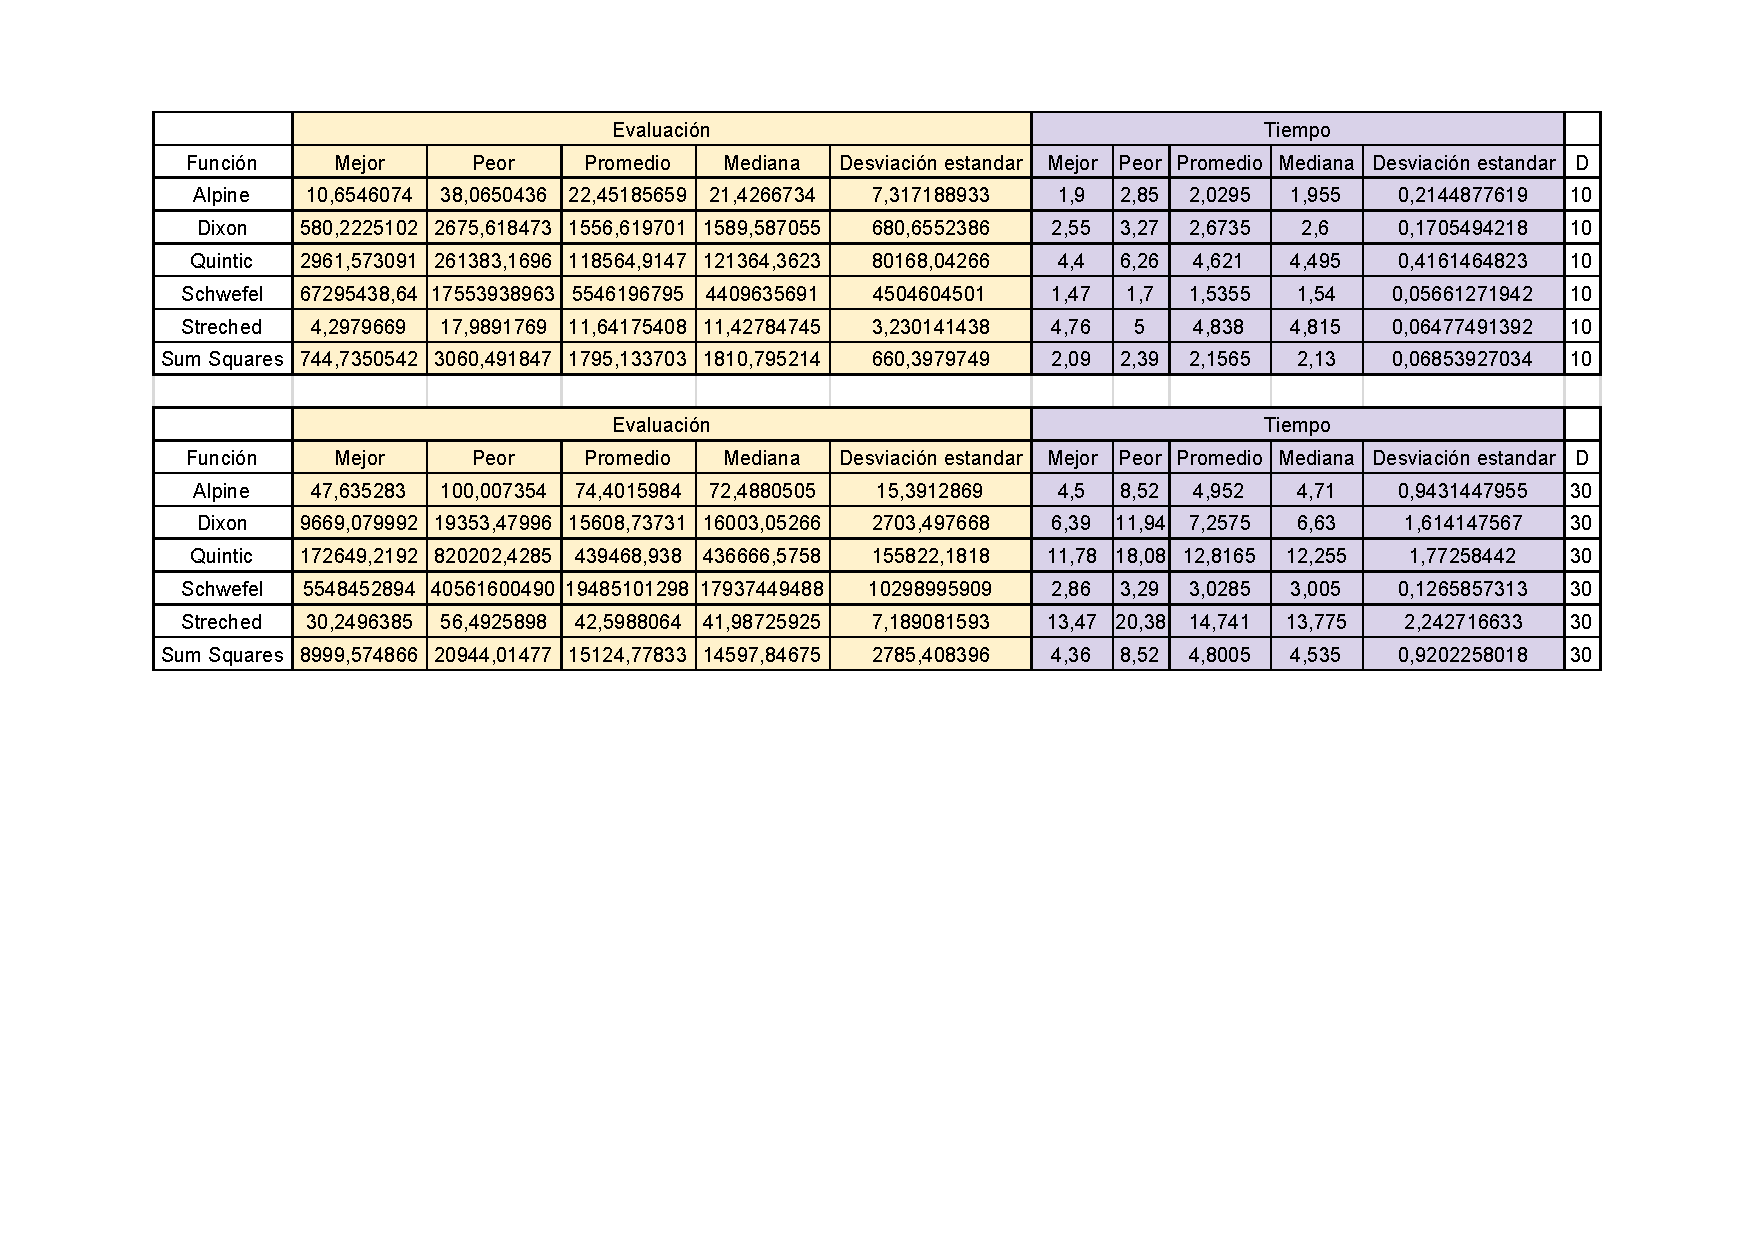
\includegraphics[scale=0.65]{docs/RMHC_SA_Metaheuristics-RMHC.pdf}
\end{center}
\begin{landscape}
  \subsection{SA}
  \begin{center}
    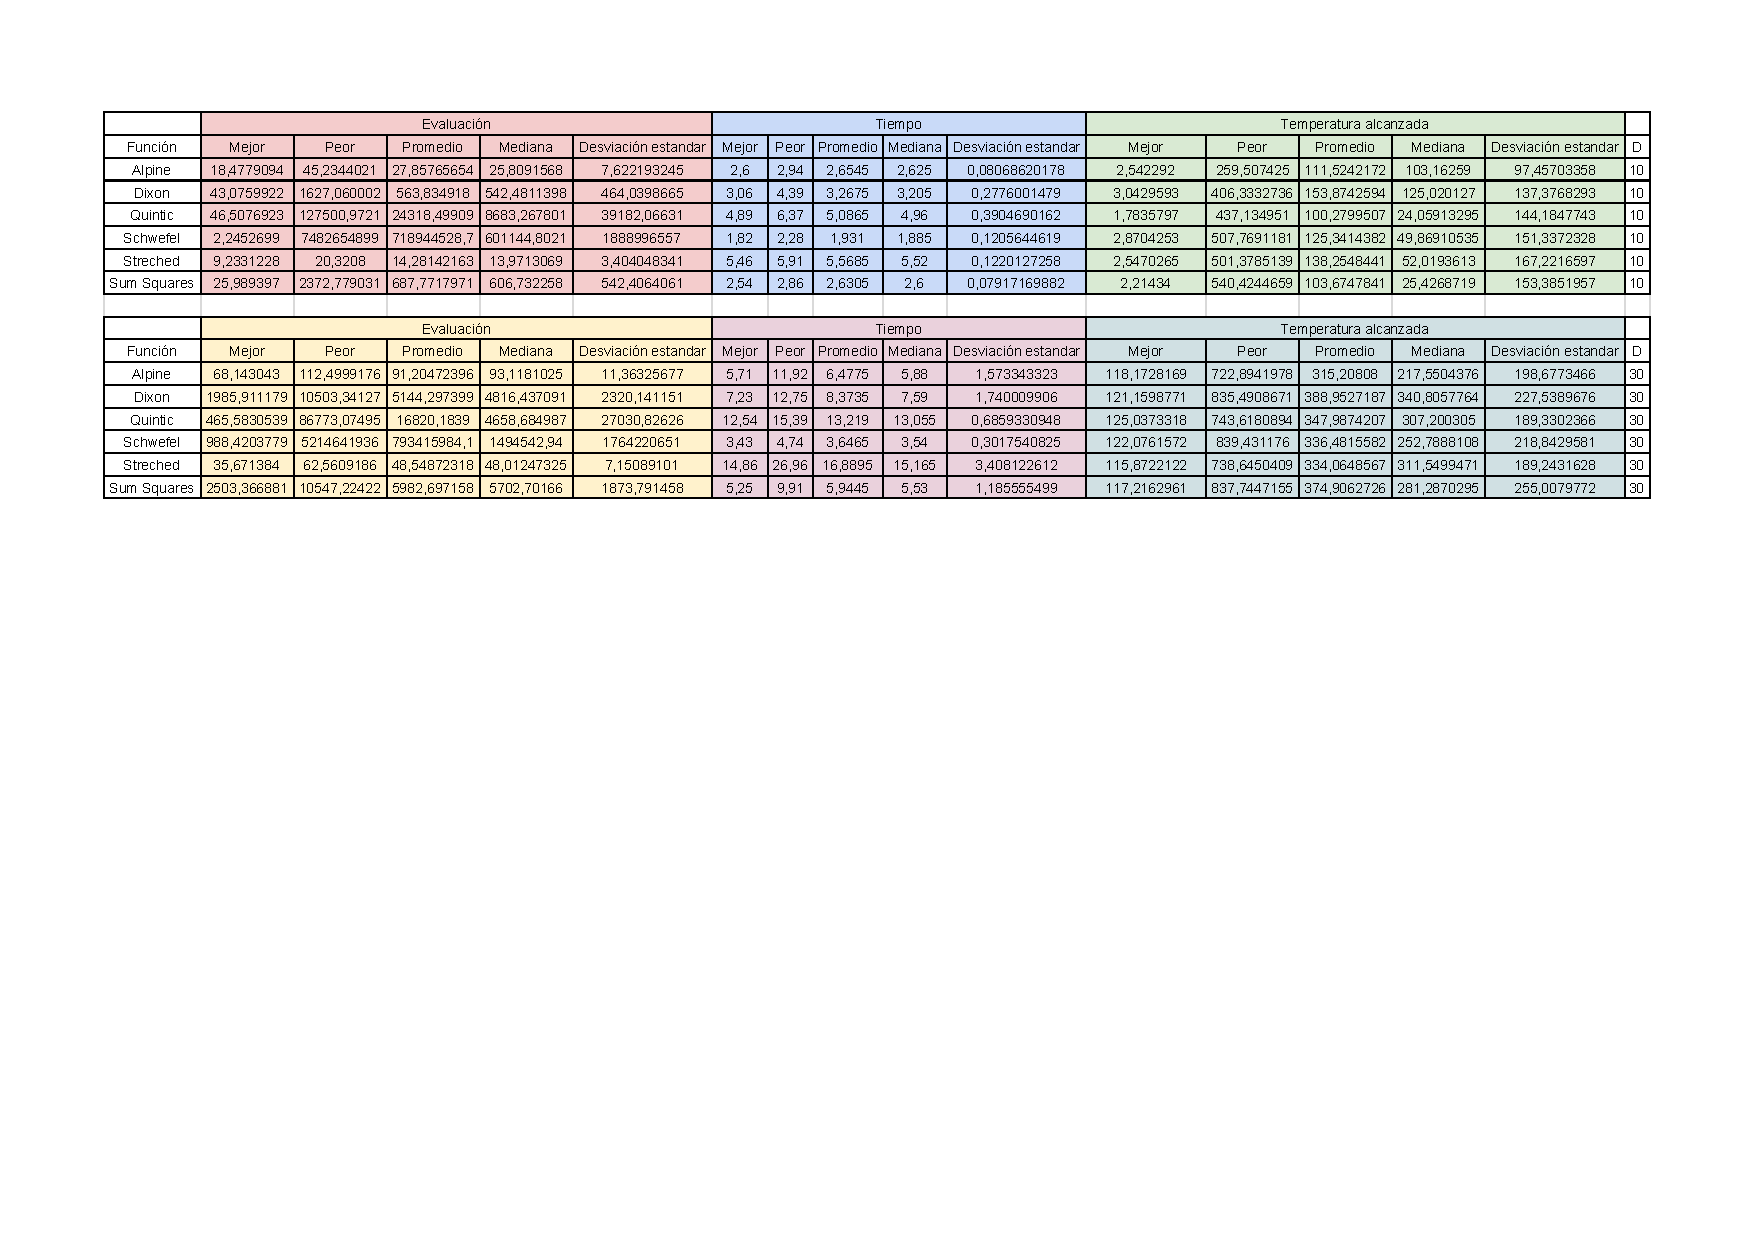
\includegraphics[scale=0.75]{docs/RMHC_SA_Metaheuristics-SA.pdf}
    \fillandplacepagenumber
  \end{center}
\end{landscape}
\subsection{Discusión respecto a la implementación RMHC y SA}
Si bien podemos ejecutar ambos algoritmos con algunas condiciones compartidas, como es el caso de compartir el máximo número de iteraciones que admite el programa y como fue indicado, la obtención de sus soluciones y por ende de los valores que retorna el programa son distintos respecto a una iteración, debido a que una vez entra una nueva iteración en la llamada del algoritmo RMHC o SA este genera una solución aleatoria que esta mostrada al menos en las tablas de SA particulares de cada función, por ello podemos que el hecho de implementar alguno de los dos algoritmos nos es conveniente saber que al menos los algoritmos actúan de forma en que la iteración $0$ genere una solución aleatoria, y sobre ella podamos evolucionar aleatoriamente o bajo el esquema de recocido, obteniendo soluciones aceptables donde al momento de ser evaluadas por la computadora estas no demoren en mostrar su valor numérico y tengan proximidad a su mínimo global o local.
\begin{landscape}
  \subsection{Tablas particulares}
  \subsubsection{Alpine}
  \begin{center}
    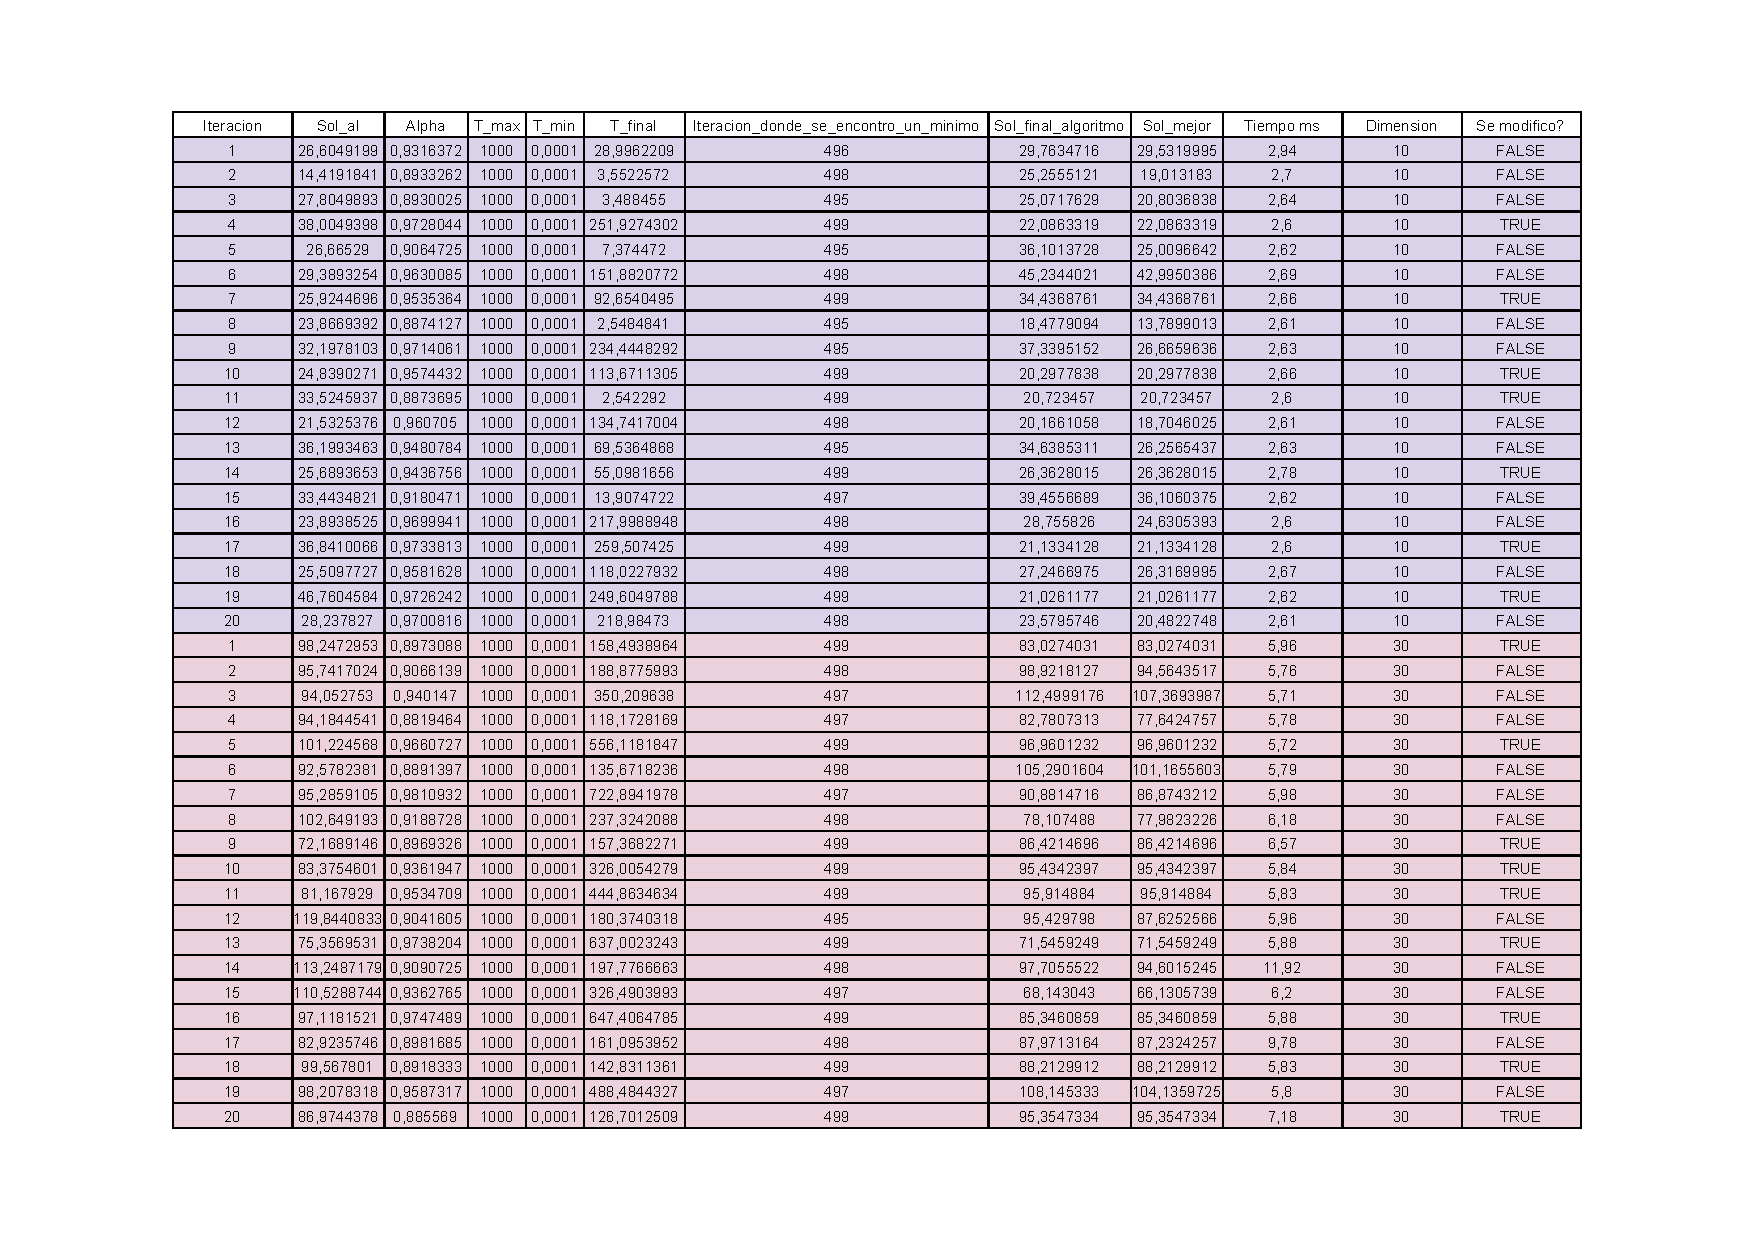
\includegraphics[scale=0.7]{docs/RMHC_SA_Metaheuristics-SA_Alpine.pdf}
  \end{center}
  \fillandplacepagenumber
  \subsubsection{Dixon}
  \begin{center}
    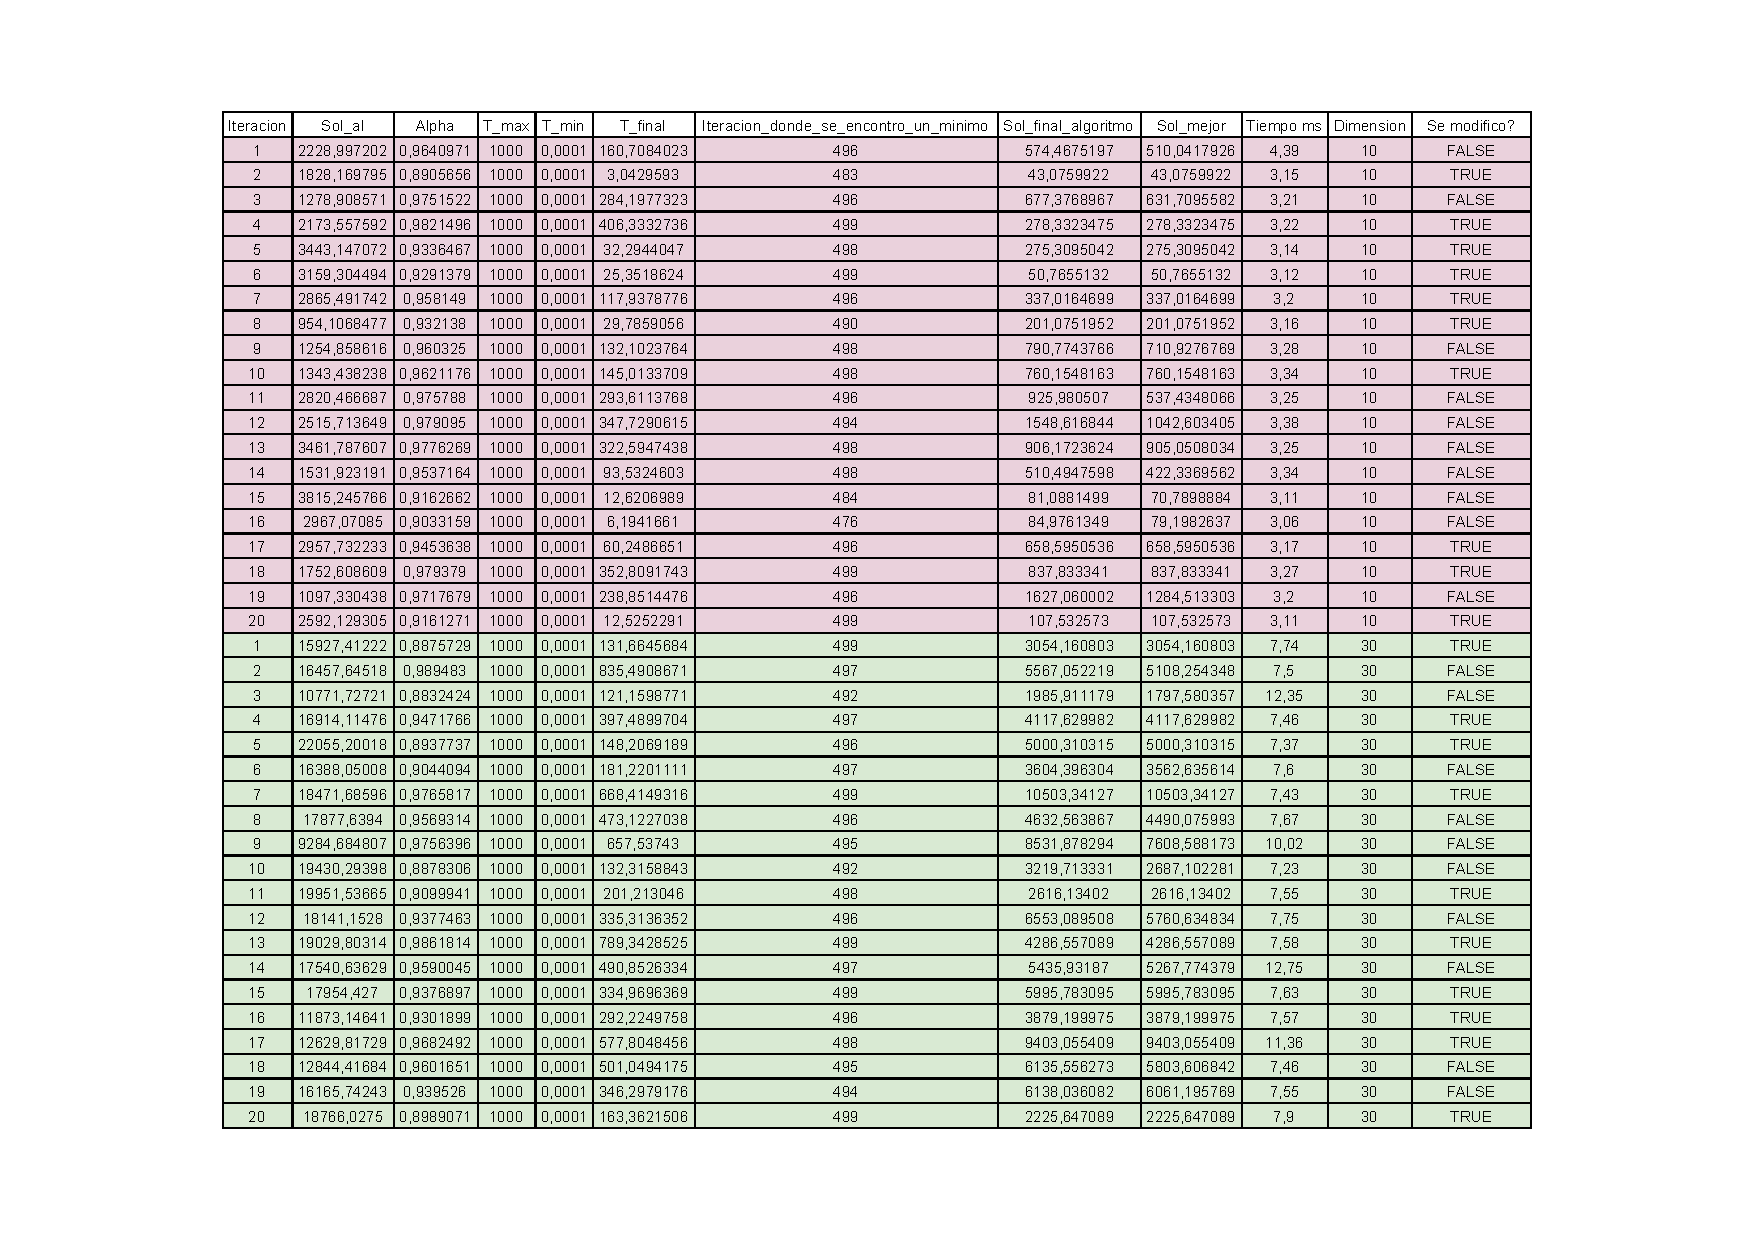
\includegraphics[scale=0.7]{docs/RMHC_SA_Metaheuristics-SA_Dixon.pdf}
  \end{center}
  \fillandplacepagenumber
  \subsubsection{Quintic}
  \begin{center}
    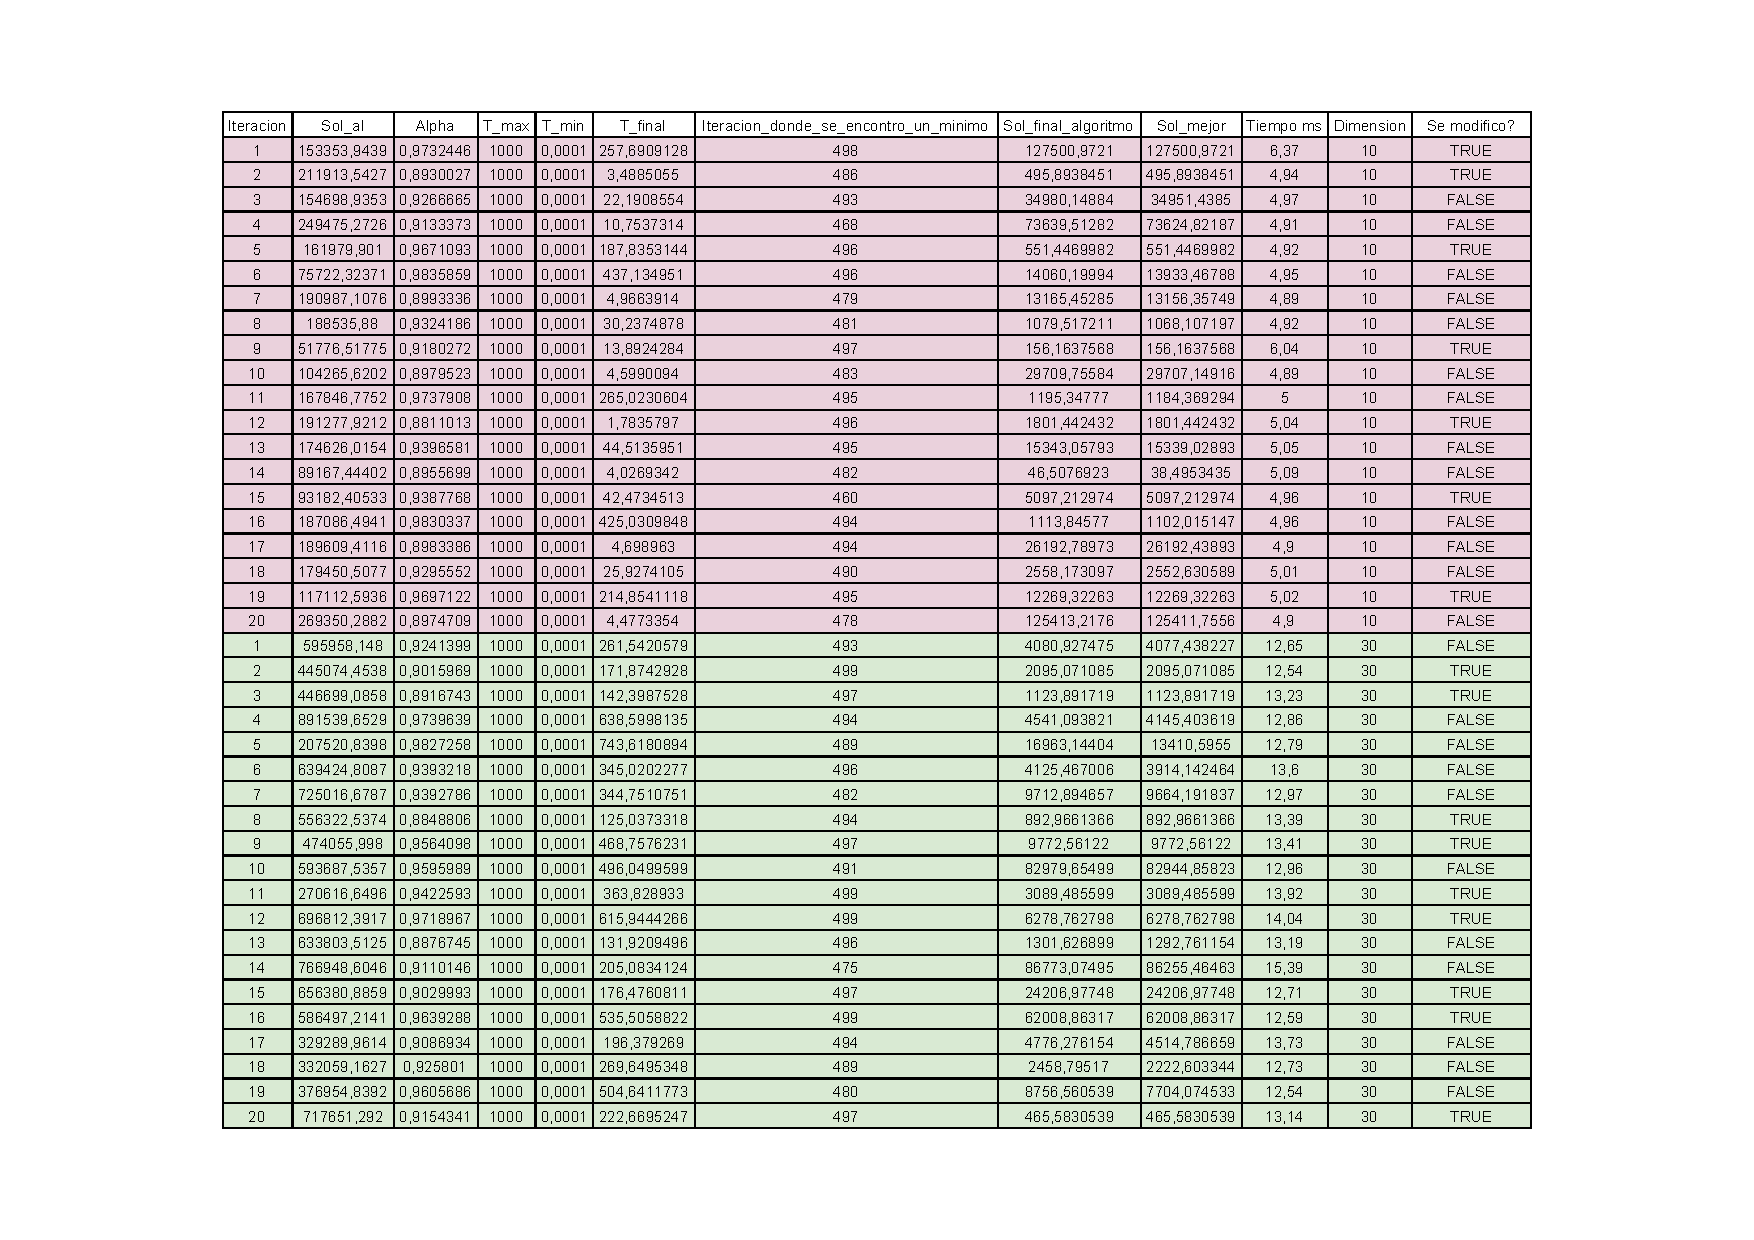
\includegraphics[scale=0.7]{docs/RMHC_SA_Metaheuristics-SA_Quintic.pdf}
  \end{center}
  \fillandplacepagenumber
  \subsubsection{Schwefel}
  \begin{center}
    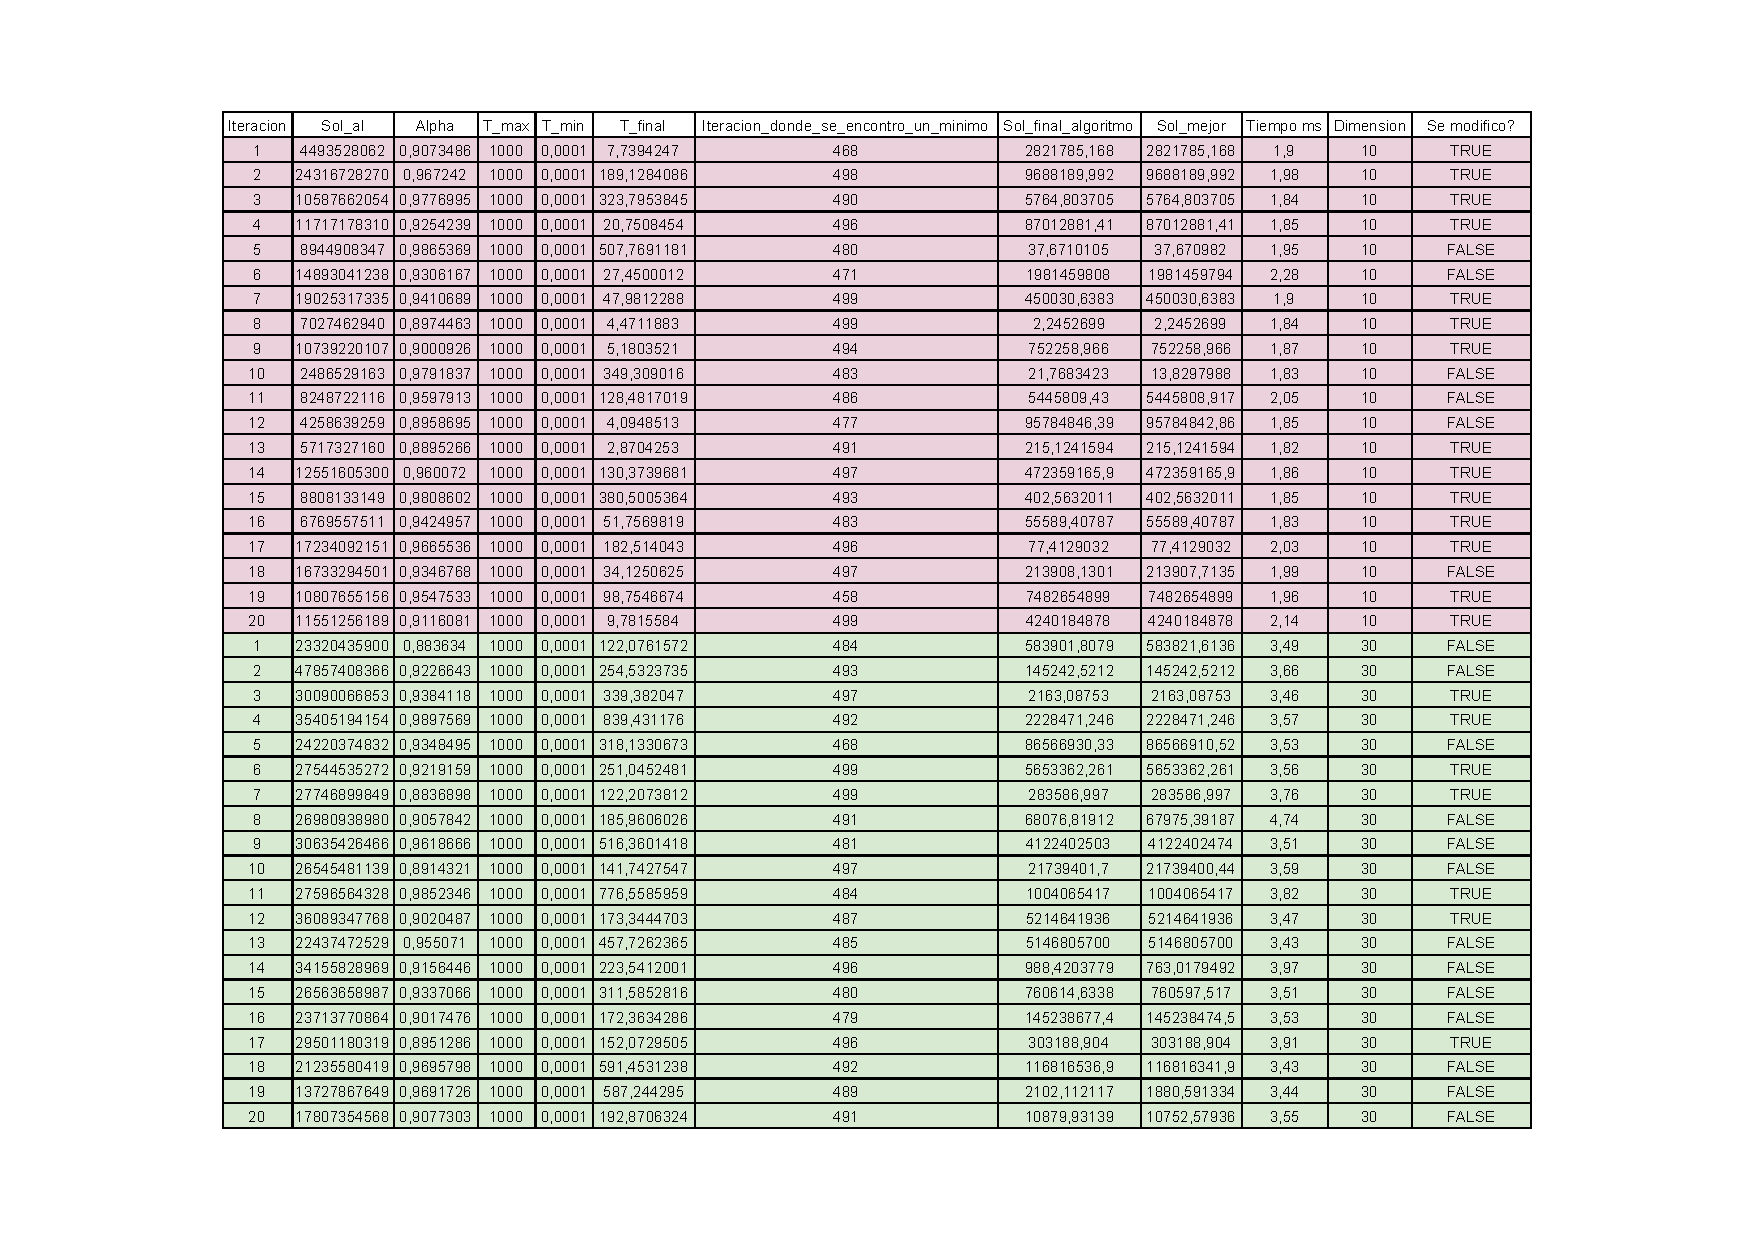
\includegraphics[scale=0.7]{docs/RMHC_SA_Metaheuristics-SA_Schwefel.pdf}
  \end{center}
  \fillandplacepagenumber
  \subsubsection{Streched}
  \begin{center}
    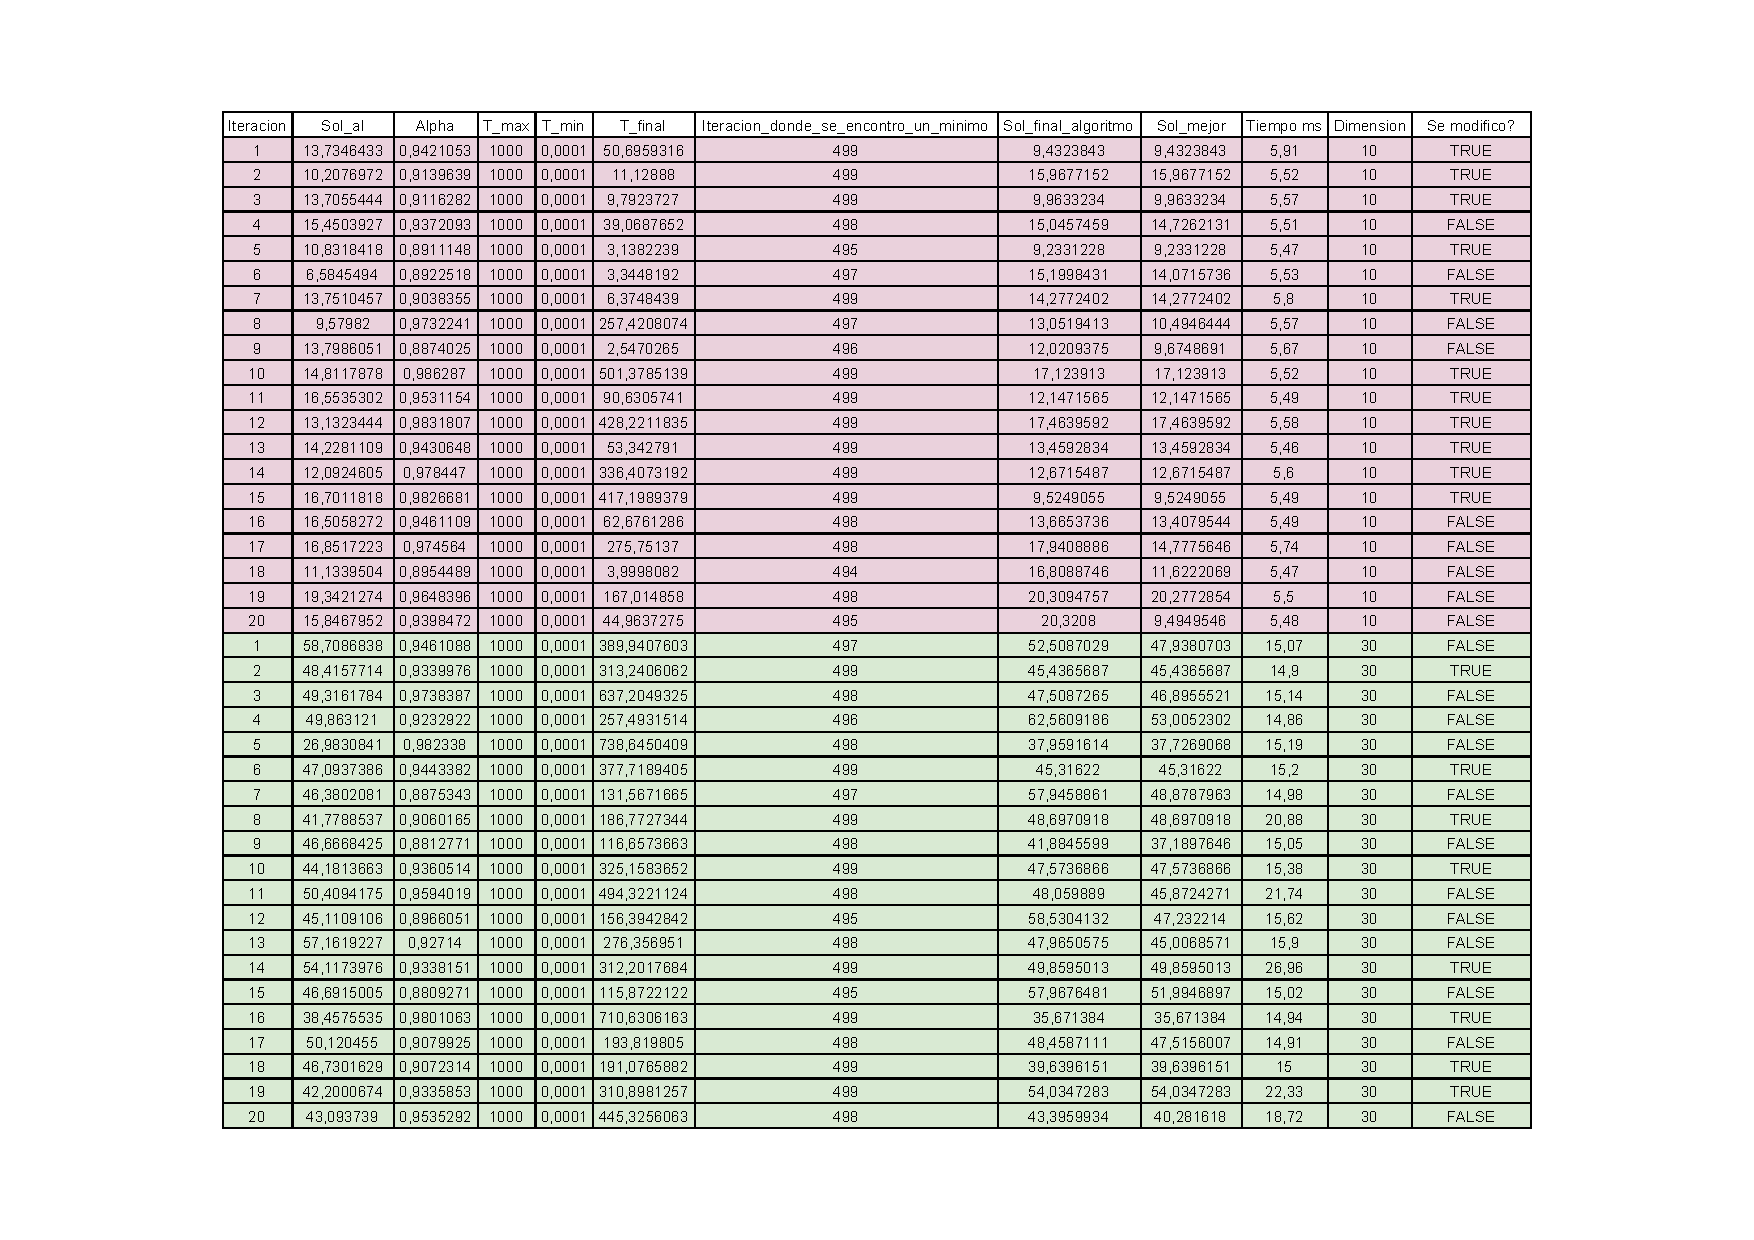
\includegraphics[scale=0.7]{docs/RMHC_SA_Metaheuristics-SA_Streched.pdf}
  \end{center}
  \fillandplacepagenumber
  \subsubsection{Sum Squares}
  \begin{center}
    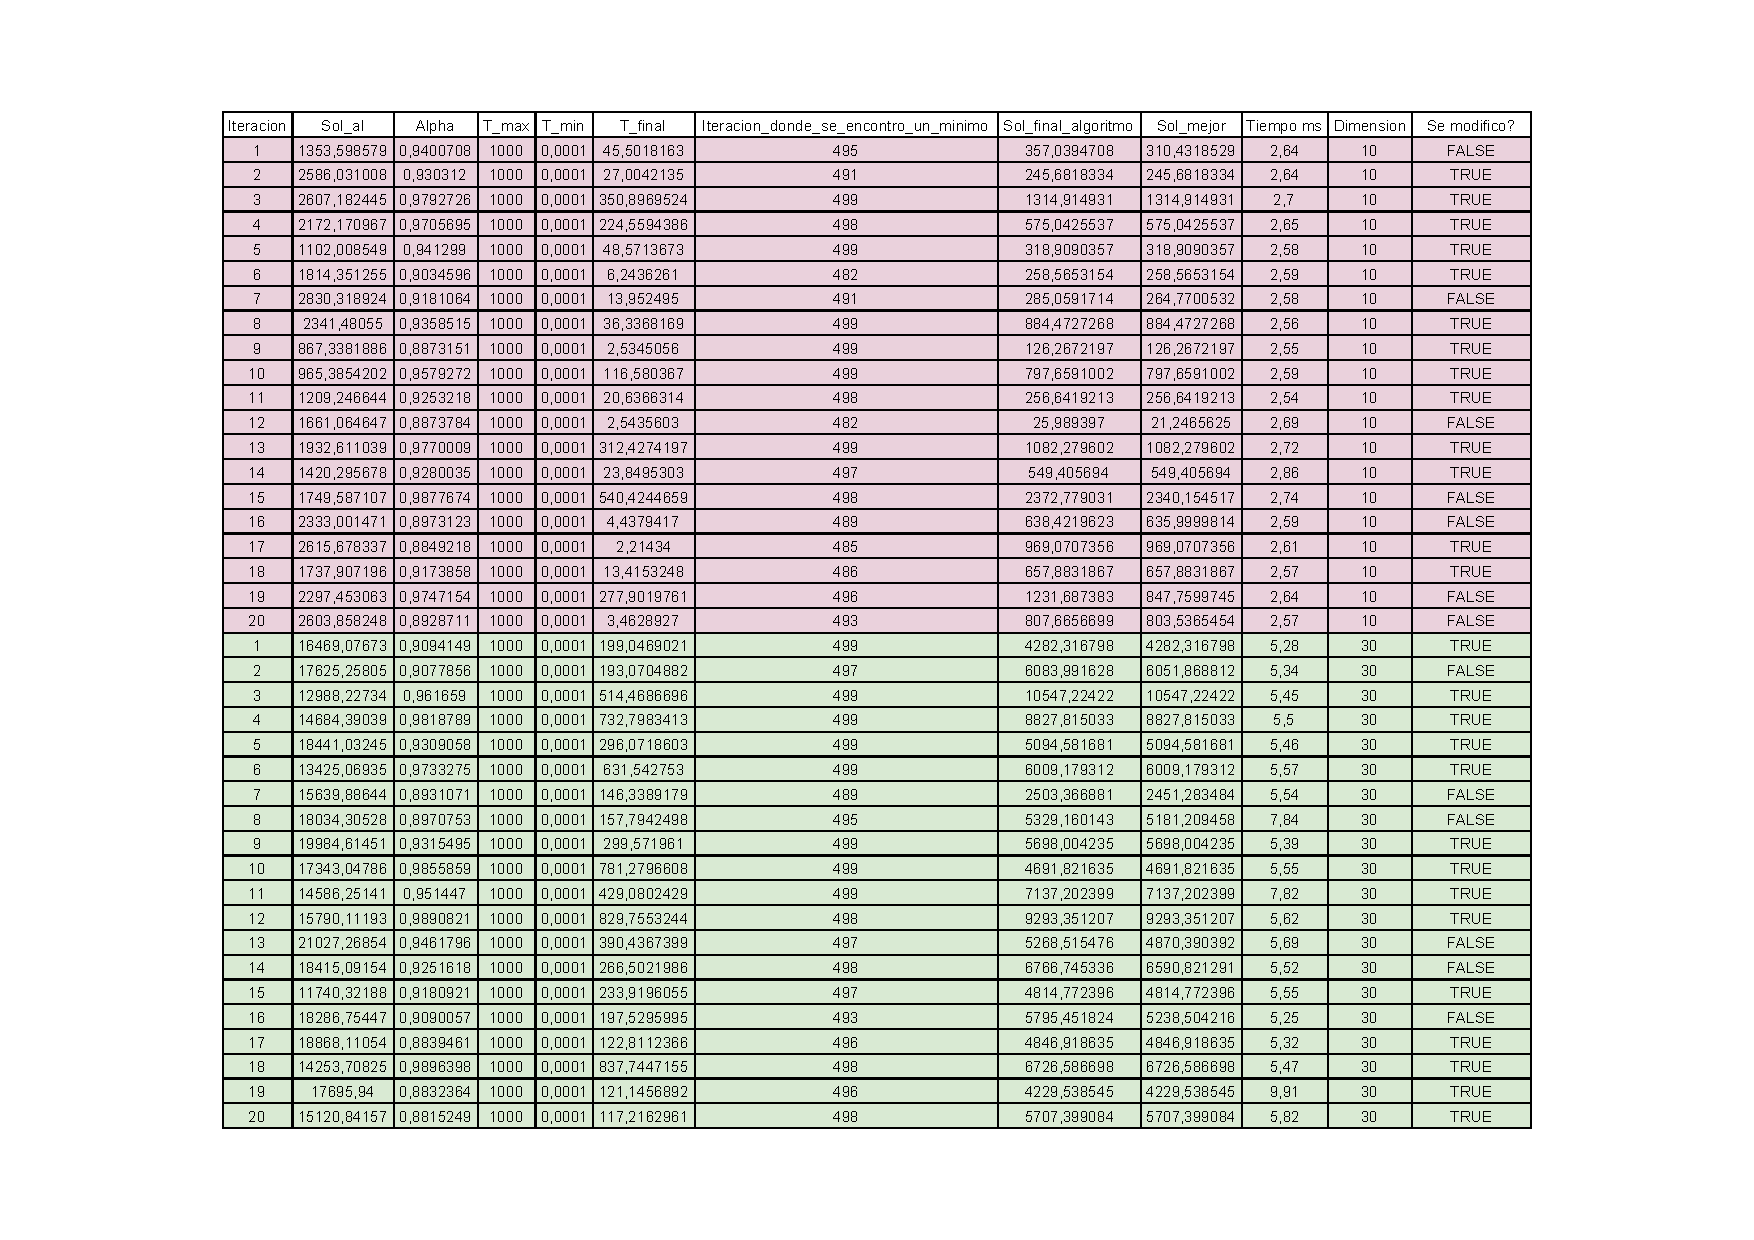
\includegraphics[scale=0.7]{docs/RMHC_SA_Metaheuristics-SA_SumSquare.pdf}
  \end{center}
  \fillandplacepagenumber
\end{landscape}
\subsection{Discusión respecto a las tablas del algoritmo SA}
Finalmente de forma detallada podemos ver los resultados y la aleatoriedad de los valores programados y obtenidos de por lo que en algunas ocasiones el mínimo obtenido se ve modificado por uno distinto al valor que obtuvimos y que era mejor, en las tablas podemos ver que en están en el sentido inverso, es decir, un valor $False$ es equivalente a decir que es un valor $Modificado$ en la solución, mientras que un valor $True$ es equivalente a $No Modificado$, por lo tanto dependiendo de nuestra función de probabilidad sea aceptable y de que el equipo genere un vecino cuya solución es peor a la solución vieja, esta modifique la solución y las siguientes iteraciones no se vean afectadas por las nuevas soluciones "mejores" a la solución que fue aceptada, por otro lado también podemos ver la forma de actuar de la aleatoriedad del valor $\alpha$ actúa de forma en que la temperatura al final de la ejecución es aceptablemente baja o en su defecto es bastante alta considerada a otras temperaturas.
\section{Conclusiones}
Los algoritmos heurísticos de trayectoria simple como son RMHC y SA, nos permiten computar y obtener soluciones aproximadas al mínimo local o global de cualquier función de optimización cuyo espacio de soluciones cae en la categoría de problemas NP y NP-Completos, por lo que podemos aproximar una solución aceptable en tiempo y recursos de memoria que nos permita comprender y analizar el espacio de soluciones de modo que al ser implementados de una forma, estos se puedan hibridar con otros algoritmos u otros problemas a optimizar.
\\
Para finalizar es importante reconocer que existen más heurísticas que permiten abordar otros problemas que no son de trayectoria simple, por lo que en un futuro, así como en los papers de investigación es posible realizar una implementación híbrida en distintos dominios (Discreto, Continuo o Discontinuo), de modo que podamos modelar y solucionar una problemática de planificación, reconocimiento de patrones y/u optimización en general.
\end{document}
